\documentclass[8pt,aspectratio=169]{beamer}
\usepackage[utf8]{inputenc}
\usepackage{graphicx}
\usepackage{amsmath,amssymb}
\usepackage{xcolor}
\usepackage{tikz}
\usepackage{multicol}
\usepackage{tcolorbox}
\usepackage{booktabs}
\usepackage{hyperref}

% Theme settings
\usetheme{Madrid}
\usecolortheme{seahorse}
\setbeamertemplate{navigation symbols}{}
\setbeamertemplate{footline}[frame number]

% Custom colors for consistency
\definecolor{darkblue}{RGB}{0,51,102}
\definecolor{lightblue}{RGB}{173,216,230}
\definecolor{accent1}{RGB}{255,107,107}  % Red for current/important
\definecolor{accent2}{RGB}{78,205,196}   % Teal for context
\definecolor{accent3}{RGB}{149,231,126}  % Green for output/success
\definecolor{accent4}{RGB}{255,195,0}    % Gold for highlights

% Custom commands
\newcommand{\highlight}[1]{\textcolor{darkblue}{\textbf{#1}}}
\newcommand{\yearmarker}[1]{\textcolor{accent1}{\textbf{#1}}}
\newcommand{\prob}[1]{P(#1)}
\newcommand{\given}{\mid}

\title[NLP Course Complete Overview]{Natural Language Processing: Complete Course Overview}
\subtitle{From Foundations to State-of-the-Art}
\author{Joerg R. Osterrieder \\ \url{www.joergosterrieder.com}}
\date{BSc Computer Science - 12 Week Journey}

\begin{document}

% Title slide
\begin{frame}
    \titlepage
\end{frame}

%============================================================================
% PART 1: COURSE-LEVEL OVERVIEW (3 slides)
%============================================================================

% Course Slide 1: The NLP Journey
\begin{frame}[t]{The NLP Journey: From Counting to Understanding}
    \centering
    \includegraphics[width=0.85\textwidth]{../figures/course_roadmap.pdf}
    
    \vspace{0.3em}
    \begin{columns}[T]
        \begin{column}{0.32\textwidth}
            \centering
            \textbf{\textcolor{accent1}{Foundation Phase}}\\
            \small Weeks 1-4\\
            \tiny
            \begin{itemize}
                \item Statistical models
                \item Neural basics
                \item Sequential processing
                \item First architectures
            \end{itemize}
        \end{column}
        \begin{column}{0.32\textwidth}
            \centering
            \textbf{\textcolor{accent2}{Revolution Phase}}\\
            \small Weeks 5-8\\
            \tiny
            \begin{itemize}
                \item Transformer breakthrough
                \item Pre-trained models
                \item Advanced architectures
                \item Tokenization mastery
            \end{itemize}
        \end{column}
        \begin{column}{0.32\textwidth}
            \centering
            \textbf{\textcolor{accent3}{Application Phase}}\\
            \small Weeks 9-12\\
            \tiny
            \begin{itemize}
                \item Decoding strategies
                \item Fine-tuning expertise
                \item Efficiency optimization
                \item Ethical deployment
            \end{itemize}
        \end{column}
    \end{columns}
    
    \vspace{0.3em}
    \begin{tcolorbox}[colback=lightblue!10,colframe=darkblue,boxrule=0.5pt]
        \centering
        \small \textbf{12 Weeks} • \textbf{3 Paradigm Shifts} • \textbf{From 0 to State-of-the-Art}
    \end{tcolorbox}
\end{frame}

% Course Slide 2: Core Technologies
\begin{frame}[t]{Core Technologies \& Breakthroughs}
    \centering
    \includegraphics[width=0.85\textwidth]{../figures/technology_evolution.pdf}
    
    \vspace{0.3em}
    \begin{columns}[T]
        \begin{column}{0.48\textwidth}
            \textbf{Major Paradigm Shifts:}
            \small
            \begin{itemize}
                \item[\yearmarker{1990s}] \textbf{Statistical Era}
                    \begin{itemize}
                        \tiny
                        \item N-grams dominate
                        \item Count-based methods
                    \end{itemize}
                \item[\yearmarker{2013}] \textbf{Embedding Revolution}
                    \begin{itemize}
                        \tiny
                        \item Word2Vec breakthrough
                        \item Semantic understanding
                    \end{itemize}
                \item[\yearmarker{2017}] \textbf{Transformer Age}
                    \begin{itemize}
                        \tiny
                        \item Attention is all you need
                        \item Parallel processing
                    \end{itemize}
                \item[\yearmarker{2020+}] \textbf{Scale \& Capability}
                    \begin{itemize}
                        \tiny
                        \item GPT-3/4, Claude, Gemini
                        \item Emergent abilities
                    \end{itemize}
            \end{itemize}
        \end{column}
        \begin{column}{0.48\textwidth}
            \textbf{Performance Leaps:}
            \small
            \begin{center}
            \begin{tabular}{lcc}
                \toprule
                \textbf{Technology} & \textbf{Year} & \textbf{Impact} \\
                \midrule
                N-grams & 1990s & Baseline \\
                Word2Vec & 2013 & 5x better \\
                Transformers & 2017 & 50x better \\
                BERT & 2018 & 100x better \\
                GPT-3 & 2020 & 1000x better \\
                GPT-4 & 2023 & 10000x better \\
                \bottomrule
            \end{tabular}
            \end{center}
            
            \vspace{0.5em}
            \begin{tcolorbox}[colback=accent4!10,colframe=accent4,boxrule=0.5pt]
                \centering
                \tiny Model parameters: 1M → 1T in 20 years
            \end{tcolorbox}
        \end{column}
    \end{columns}
\end{frame}

% Course Slide 3: Learning Outcomes
\begin{frame}[t]{Learning Outcomes \& Real-World Impact}
    \centering
    \includegraphics[width=0.85\textwidth]{../figures/skills_applications.pdf}
    
    \vspace{0.3em}
    \begin{columns}[T]
        \begin{column}{0.32\textwidth}
            \textbf{\textcolor{accent1}{Core Skills}}
            \small
            \begin{itemize}
                \item Implement transformers
                \item Fine-tune BERT/GPT
                \item Build chat systems
                \item Deploy models
                \item Optimize efficiency
                \item Ensure fairness
            \end{itemize}
        \end{column}
        \begin{column}{0.32\textwidth}
            \textbf{\textcolor{accent2}{Technologies}}
            \small
            \begin{itemize}
                \item PyTorch/TensorFlow
                \item Hugging Face
                \item LangChain
                \item ONNX/TensorRT
                \item Docker/Kubernetes
                \item MLOps tools
            \end{itemize}
        \end{column}
        \begin{column}{0.32\textwidth}
            \textbf{\textcolor{accent3}{Applications}}
            \small
            \begin{itemize}
                \item ChatGPT-like systems
                \item Translation services
                \item Code assistants
                \item Content generation
                \item Search engines
                \item Virtual assistants
            \end{itemize}
        \end{column}
    \end{columns}
    
    \vspace{0.3em}
    \begin{columns}[T]
        \begin{column}{0.48\textwidth}
            \begin{tcolorbox}[colback=accent1!10,colframe=accent1,boxrule=0.5pt]
                \centering
                \textbf{Industry Demand}\\
                \small NLP Engineers: \textbf{\$150k-300k}\\
                \tiny 10,000+ open positions globally
            \end{tcolorbox}
        \end{column}
        \begin{column}{0.48\textwidth}
            \begin{tcolorbox}[colback=accent3!10,colframe=accent3,boxrule=0.5pt]
                \centering
                \textbf{Market Impact}\\
                \small NLP Market: \textbf{\$43B by 2025}\\
                \tiny 20\% annual growth rate
            \end{tcolorbox}
        \end{column}
    \end{columns}
\end{frame}

%============================================================================
% WEEK 1: FOUNDATIONS (3 slides)
%============================================================================

\section{Week 1: Foundations}

\begin{frame}[t]{Week 1: What We'll Learn}
    \centering
    \includegraphics[width=0.85\textwidth]{../../week01_foundations/figures/week1_learning_objectives.pdf}
    
    \vspace{0.3em}
    \begin{columns}[T]
        \begin{column}{0.48\textwidth}
            \textbf{\textcolor{accent1}{Core Concepts:}}
            \small
            \begin{itemize}
                \item \textbf{Probability Theory} for NLP
                    \begin{itemize}
                        \tiny
                        \item Joint, conditional, marginal
                        \item Bayes' theorem
                        \item Maximum likelihood
                    \end{itemize}
                \item \textbf{N-gram Models}
                    \begin{itemize}
                        \tiny
                        \item Unigrams, bigrams, trigrams
                        \item Markov assumption
                        \item Language model training
                    \end{itemize}
            \end{itemize}
        \end{column}
        \begin{column}{0.48\textwidth}
            \textbf{\textcolor{accent2}{Skills You'll Gain:}}
            \small
            \begin{itemize}
                \item Calculate n-gram probabilities
                \item Build statistical language models
                \item Handle data sparsity
                \item Implement smoothing
                \item Evaluate perplexity
                \item Generate text
            \end{itemize}
        \end{column}
    \end{columns}
\end{frame}

\begin{frame}[t]{Week 1: N-gram Language Models}
    \centering
    \includegraphics[width=0.85\textwidth]{../../week01_foundations/figures/week1_ngram_concept.pdf}
    
    \vspace{0.3em}
    \begin{columns}[T]
        \begin{column}{0.32\textwidth}
            \textbf{\textcolor{accent1}{Markov Assumption}}
            \small
            \begin{itemize}
                \item Future depends on recent past
                \item Makes computation tractable
            \end{itemize}
        \end{column}
        \begin{column}{0.32\textwidth}
            \textbf{\textcolor{accent2}{Probability}}
            \small
            \begin{itemize}
                \item Count n-grams
                \item Maximum likelihood
            \end{itemize}
        \end{column}
        \begin{column}{0.32\textwidth}
            \textbf{\textcolor{accent3}{Challenges}}
            \small
            \begin{itemize}
                \item Data sparsity
                \item Context limitations
            \end{itemize}
        \end{column}
    \end{columns}
\end{frame}

\begin{frame}[t]{Week 1: Applications}
    \centering
    \includegraphics[width=0.85\textwidth]{../../week01_foundations/figures/week1_applications.pdf}
    
    \vspace{0.3em}
    \begin{columns}[T]
        \begin{column}{0.48\textwidth}
            \textbf{\textcolor{accent1}{Where N-grams Excel:}}
            \small
            \begin{itemize}
                \item Spell checking
                \item Auto-complete
                \item Speech recognition
                \item Machine translation
                \item Text generation
            \end{itemize}
        \end{column}
        \begin{column}{0.48\textwidth}
            \textbf{\textcolor{accent2}{Historical Impact:}}
            \small
            \begin{itemize}
                \item Dominated 1980s-2000s
                \item Still used in hybrid systems
                \item Baseline for evaluation
                \item Foundation for understanding
            \end{itemize}
        \end{column}
    \end{columns}
\end{frame}

%============================================================================
% WEEK 2: NEURAL LM & EMBEDDINGS (3 slides)
%============================================================================

\section{Week 2: Neural Language Models}

\begin{frame}[t]{Week 2: Neural Revolution}
    \centering
    \includegraphics[width=0.85\textwidth]{../../week02_neural_lm/figures/week2_neural_evolution.pdf}
    
    \vspace{0.3em}
    \begin{columns}[T]
        \begin{column}{0.48\textwidth}
            \textbf{\textcolor{accent1}{Paradigm Shift:}}
            \small
            \begin{itemize}
                \item From counting to learning
                \item Continuous space
                \item Neural architecture
                \item Generalization power
            \end{itemize}
        \end{column}
        \begin{column}{0.48\textwidth}
            \textbf{\textcolor{accent2}{Key Innovations:}}
            \small
            \begin{itemize}
                \item Distributed representations
                \item Backpropagation training
                \item Parameter sharing
                \item Transfer learning
            \end{itemize}
        \end{column}
    \end{columns}
\end{frame}

\begin{frame}[t]{Week 2: Word Embeddings}
    \centering
    \includegraphics[width=0.85\textwidth]{../../week02_neural_lm/figures/week2_embedding_space.pdf}
    
    \vspace{0.3em}
    \begin{columns}[T]
        \begin{column}{0.32\textwidth}
            \textbf{\textcolor{accent1}{Properties}}
            \small
            \begin{itemize}
                \item Similar words cluster
                \item Analogies work
            \end{itemize}
        \end{column}
        \begin{column}{0.32\textwidth}
            \textbf{\textcolor{accent2}{Methods}}
            \small
            \begin{itemize}
                \item Word2Vec
                \item GloVe, FastText
            \end{itemize}
        \end{column}
        \begin{column}{0.32\textwidth}
            \textbf{\textcolor{accent3}{Dimensions}}
            \small
            \begin{itemize}
                \item 50-300 dims typical
                \item Semantic features
            \end{itemize}
        \end{column}
    \end{columns}
\end{frame}

\begin{frame}[t]{Week 2: Impact}
    \centering
    \includegraphics[width=0.85\textwidth]{../../week02_neural_lm/figures/week2_applications_impact.pdf}
    
    \vspace{0.3em}
    \begin{columns}[T]
        \begin{column}{0.48\textwidth}
            \textbf{\textcolor{accent1}{Algorithms:}}
            \small
            \begin{itemize}
                \item CBOW: Context → center
                \item Skip-gram: Center → context
                \item Negative sampling
            \end{itemize}
        \end{column}
        \begin{column}{0.48\textwidth}
            \textbf{\textcolor{accent2}{Applications:}}
            \small
            \begin{itemize}
                \item Sentiment analysis
                \item Named entity recognition
                \item Text classification
            \end{itemize}
        \end{column}
    \end{columns}
\end{frame}

%============================================================================
% WEEK 3: RNN/LSTM/GRU (3 slides)
%============================================================================

\section{Week 3: Recurrent Neural Networks}

\begin{frame}[t]{Week 3: Sequential Processing}
    \centering
    \includegraphics[width=0.85\textwidth]{../../figures/rnn_sequential_bottleneck.pdf}
    
    \vspace{0.3em}
    \begin{columns}[T]
        \begin{column}{0.48\textwidth}
            \textbf{\textcolor{accent1}{What We'll Learn:}}
            \small
            \begin{itemize}
                \item RNN architecture
                \item LSTM gates and memory
                \item GRU simplifications
                \item Backpropagation through time
                \item Bidirectional processing
            \end{itemize}
            
            \vspace{0.5em}
            \textbf{Key Innovation:}
            \small
            \begin{itemize}
                \item Hidden state maintains context
                \item Process sequences of any length
                \item Share parameters across time
            \end{itemize}
        \end{column}
        \begin{column}{0.48\textwidth}
            \textbf{\textcolor{accent2}{Core Concepts:}}
            \small
            \begin{itemize}
                \item \textbf{Vanishing Gradients}
                    \begin{itemize}
                        \tiny
                        \item Problem with long sequences
                        \item LSTM/GRU solutions
                    \end{itemize}
                \item \textbf{Gate Mechanisms}
                    \begin{itemize}
                        \tiny
                        \item Forget gate
                        \item Input gate
                        \item Output gate
                    \end{itemize}
                \item \textbf{Memory Cells}
                    \begin{itemize}
                        \tiny
                        \item Long-term dependencies
                        \item Selective memory
                    \end{itemize}
            \end{itemize}
        \end{column}
    \end{columns}
\end{frame}

\begin{frame}[t]{Week 3: LSTM Architecture}
    \centering
    \includegraphics[width=0.85\textwidth]{../../figures/lstm_gates_intuitive.pdf}
    
    \vspace{0.3em}
    \begin{columns}[T]
        \begin{column}{0.32\textwidth}
            \textbf{\textcolor{accent1}{Information Flow}}
            \small
            \begin{itemize}
                \item Cell state highway
                \item Gated updates
                \item Selective forgetting
            \end{itemize}
        \end{column}
        \begin{column}{0.32\textwidth}
            \textbf{\textcolor{accent2}{Advantages}}
            \small
            \begin{itemize}
                \item Captures long-range
                \item Stable gradients
                \item Flexible memory
            \end{itemize}
        \end{column}
        \begin{column}{0.32\textwidth}
            \textbf{\textcolor{accent3}{Limitations}}
            \small
            \begin{itemize}
                \item Sequential processing
                \item Cannot parallelize
                \item Slow training
            \end{itemize}
        \end{column}
    \end{columns}
    
    \vspace{0.5em}
    \begin{tcolorbox}[colback=lightblue!10,colframe=darkblue,boxrule=0.5pt]
        \centering
        \small RNNs dominated sequence modeling from 2010-2017
    \end{tcolorbox}
\end{frame}

\begin{frame}[t]{Week 3: Applications}
    \centering
    \includegraphics[width=0.85\textwidth]{../../figures/rnn_vs_lstm_performance.pdf}
    
    \vspace{0.3em}
    \begin{columns}[T]
        \begin{column}{0.48\textwidth}
            \textbf{\textcolor{accent1}{Tasks:}}
            \small
            \begin{itemize}
                \item Named Entity Recognition
                \item Part-of-Speech Tagging
                \item Sentiment Analysis
                \item Time Series Prediction
                \item Speech Recognition
            \end{itemize}
        \end{column}
        \begin{column}{0.48\textwidth}
            \textbf{\textcolor{accent2}{Performance:}}
            \small
            \begin{itemize}
                \item State-of-art until 2017
                \item Good for online processing
                \item Memory efficient
                \item Still used for streaming
            \end{itemize}
        \end{column}
    \end{columns}
\end{frame}

%============================================================================
% WEEK 4: SEQ2SEQ (3 slides)
%============================================================================

\section{Week 4: Sequence-to-Sequence}

\begin{frame}[t]{Week 4: Encoder-Decoder Architecture}
    \centering
    \includegraphics[width=0.85\textwidth]{../../figures/seq2seq_architecture.pdf}
    
    \vspace{0.3em}
    \begin{columns}[T]
        \begin{column}{0.48\textwidth}
            \textbf{\textcolor{accent1}{What We'll Learn:}}
            \small
            \begin{itemize}
                \item Encoder-decoder paradigm
                \item Context vectors
                \item Attention mechanism
                \item Beam search decoding
                \item Teacher forcing
            \end{itemize}
        \end{column}
        \begin{column}{0.48\textwidth}
            \textbf{\textcolor{accent2}{Key Concepts:}}
            \small
            \begin{itemize}
                \item Information bottleneck
                \item Variable length I/O
                \item Cross-attention
                \item Alignment learning
            \end{itemize}
        \end{column}
    \end{columns}
\end{frame}

\begin{frame}[t]{Week 4: Attention Mechanism}
    \centering
    \includegraphics[width=0.85\textwidth]{../../figures/attention_heatmap.pdf}
    
    \vspace{0.3em}
    \begin{columns}[T]
        \begin{column}{0.32\textwidth}
            \textbf{\textcolor{accent1}{Problem}}
            \small
            \begin{itemize}
                \item Fixed context vector
                \item Information loss
                \item Poor on long sequences
            \end{itemize}
        \end{column}
        \begin{column}{0.32\textwidth}
            \textbf{\textcolor{accent2}{Solution}}
            \small
            \begin{itemize}
                \item Dynamic context
                \item Attention weights
                \item Direct connections
            \end{itemize}
        \end{column}
        \begin{column}{0.32\textwidth}
            \textbf{\textcolor{accent3}{Impact}}
            \small
            \begin{itemize}
                \item Better translation
                \item Interpretability
                \item Path to Transformers
            \end{itemize}
        \end{column}
    \end{columns}
\end{frame}

\begin{frame}[t]{Week 4: Applications}
    \centering
    \includegraphics[width=0.85\textwidth]{../../figures/seq2seq_performance.pdf}
    
    \vspace{0.3em}
    \begin{columns}[T]
        \begin{column}{0.48\textwidth}
            \textbf{\textcolor{accent1}{Tasks:}}
            \small
            \begin{itemize}
                \item Machine Translation
                \item Text Summarization
                \item Dialogue Systems
                \item Image Captioning
                \item Speech Recognition
            \end{itemize}
        \end{column}
        \begin{column}{0.48\textwidth}
            \textbf{\textcolor{accent2}{Metrics:}}
            \small
            \begin{itemize}
                \item BLEU scores improved 10x
                \item Human-level translation
                \item Real-time processing
                \item Production deployment
            \end{itemize}
        \end{column}
    \end{columns}
\end{frame}

%============================================================================
% WEEK 5: TRANSFORMERS (3 slides)
%============================================================================

\section{Week 5: Transformers}

\begin{frame}[t]{Week 5: Attention Is All You Need}
    \centering
    \includegraphics[width=0.85\textwidth]{../../figures/transformer_architecture_detailed.pdf}
    
    \vspace{0.3em}
    \begin{columns}[T]
        \begin{column}{0.48\textwidth}
            \textbf{\textcolor{accent1}{What We'll Learn:}}
            \small
            \begin{itemize}
                \item Self-attention mechanism
                \item Multi-head attention
                \item Positional encoding
                \item Layer normalization
                \item Residual connections
            \end{itemize}
            
            \vspace{0.5em}
            \textbf{Key Innovation:}
            \small
            \begin{itemize}
                \item Fully parallel processing
                \item No recurrence needed
                \item Global context access
            \end{itemize}
        \end{column}
        \begin{column}{0.48\textwidth}
            \textbf{\textcolor{accent2}{Architecture:}}
            \small
            \begin{itemize}
                \item \textbf{Encoder Stack}
                    \begin{itemize}
                        \tiny
                        \item 6 identical layers
                        \item Self-attention + FFN
                    \end{itemize}
                \item \textbf{Decoder Stack}
                    \begin{itemize}
                        \tiny
                        \item Masked self-attention
                        \item Cross-attention
                    \end{itemize}
                \item \textbf{Scaled Dot-Product}
                    \begin{itemize}
                        \tiny
                        \item Query, Key, Value
                        \item $\sqrt{d_k}$ scaling
                    \end{itemize}
            \end{itemize}
        \end{column}
    \end{columns}
\end{frame}

\begin{frame}[t]{Week 5: Multi-Head Attention}
    \centering
    \includegraphics[width=0.85\textwidth]{../../figures/multihead_attention_patterns.pdf}
    
    \vspace{0.3em}
    \begin{columns}[T]
        \begin{column}{0.32\textwidth}
            \textbf{\textcolor{accent1}{Design}}
            \small
            \begin{itemize}
                \item 8 attention heads
                \item Different representations
                \item Concatenate \& project
            \end{itemize}
        \end{column}
        \begin{column}{0.32\textwidth}
            \textbf{\textcolor{accent2}{Benefits}}
            \small
            \begin{itemize}
                \item Multiple relationships
                \item Richer representations
                \item Better performance
            \end{itemize}
        \end{column}
        \begin{column}{0.32\textwidth}
            \textbf{\textcolor{accent3}{Efficiency}}
            \small
            \begin{itemize}
                \item O(n²) complexity
                \item Parallelizable
                \item GPU-friendly
            \end{itemize}
        \end{column}
    \end{columns}
\end{frame}

\begin{frame}[t]{Week 5: Impact}
    \centering
    \includegraphics[width=0.85\textwidth]{../../figures/transformer_vs_rnn_performance.pdf}
    
    \vspace{0.3em}
    \begin{columns}[T]
        \begin{column}{0.48\textwidth}
            \textbf{\textcolor{accent1}{Performance:}}
            \small
            \begin{itemize}
                \item SOTA on all NLP tasks
                \item 100x faster training
                \item Scales to billions of parameters
                \item Transfer learning enabled
            \end{itemize}
        \end{column}
        \begin{column}{0.48\textwidth}
            \textbf{\textcolor{accent2}{Applications:}}
            \small
            \begin{itemize}
                \item Foundation for BERT/GPT
                \item Computer Vision (ViT)
                \item Protein Folding
                \item Multimodal models
            \end{itemize}
        \end{column}
    \end{columns}
\end{frame}

%============================================================================
% WEEK 6: BERT & GPT (3 slides)
%============================================================================

\section{Week 6: Pre-trained Models}

\begin{frame}[t]{Week 6: BERT and GPT}
    \centering
    \includegraphics[width=0.85\textwidth]{../../figures/pretraining_timeline.pdf}
    
    \vspace{0.3em}
    \begin{columns}[T]
        \begin{column}{0.48\textwidth}
            \textbf{\textcolor{accent1}{What We'll Learn:}}
            \small
            \begin{itemize}
                \item Transfer learning paradigm
                \item Masked language modeling
                \item Autoregressive generation
                \item Fine-tuning strategies
                \item Model architectures
            \end{itemize}
        \end{column}
        \begin{column}{0.48\textwidth}
            \textbf{\textcolor{accent2}{Key Concepts:}}
            \small
            \begin{itemize}
                \item Unsupervised pre-training
                \item Task-specific fine-tuning
                \item Bidirectional vs unidirectional
                \item Tokenization strategies
            \end{itemize}
        \end{column}
    \end{columns}
\end{frame}

\begin{frame}[t]{Week 6: BERT vs GPT}
    \centering
    \includegraphics[width=0.85\textwidth]{../../figures/bert_vs_gpt_architecture.pdf}
    
    \vspace{0.3em}
    \begin{columns}[T]
        \begin{column}{0.48\textwidth}
            \textbf{\textcolor{accent1}{BERT (Bidirectional):}}
            \small
            \begin{itemize}
                \item Masked Language Model
                \item Sees full context
                \item Better for understanding
                \item Classification tasks
                \item 340M parameters
            \end{itemize}
        \end{column}
        \begin{column}{0.48\textwidth}
            \textbf{\textcolor{accent2}{GPT (Autoregressive):}}
            \small
            \begin{itemize}
                \item Next token prediction
                \item Left-to-right only
                \item Better for generation
                \item Creative tasks
                \item 1.5B → 175B parameters
            \end{itemize}
        \end{column}
    \end{columns}
\end{frame}

\begin{frame}[t]{Week 6: Impact}
    \centering
    \includegraphics[width=0.85\textwidth]{../../figures/bert_results_glue.pdf}
    
    \vspace{0.3em}
    \begin{columns}[T]
        \begin{column}{0.48\textwidth}
            \textbf{\textcolor{accent1}{Performance:}}
            \small
            \begin{itemize}
                \item GLUE benchmark SOTA
                \item Human-level on many tasks
                \item Few-shot learning
                \item Zero-shot capabilities
            \end{itemize}
        \end{column}
        \begin{column}{0.48\textwidth}
            \textbf{\textcolor{accent2}{Ecosystem:}}
            \small
            \begin{itemize}
                \item Hugging Face hub
                \item 100,000+ models
                \item Easy fine-tuning
                \item Production ready
            \end{itemize}
        \end{column}
    \end{columns}
\end{frame}

%============================================================================
% WEEK 7: ADVANCED TRANSFORMERS (3 slides)
%============================================================================

\section{Week 7: Advanced Transformers}

\begin{frame}[t]{Week 7: Scaling Laws and Giant Models}
    \centering
    \includegraphics[width=0.85\textwidth]{../../figures/model_scale_timeline.pdf}
    
    \vspace{0.3em}
    \begin{columns}[T]
        \begin{column}{0.48\textwidth}
            \textbf{\textcolor{accent1}{What We'll Learn:}}
            \small
            \begin{itemize}
                \item Scaling laws
                \item GPT-3/4 architecture
                \item T5 unified framework
                \item Emergent abilities
                \item Prompt engineering
            \end{itemize}
        \end{column}
        \begin{column}{0.48\textwidth}
            \textbf{\textcolor{accent2}{Model Zoo:}}
            \small
            \begin{itemize}
                \item GPT-3: 175B params
                \item T5: Text-to-text
                \item BART: Denoising
                \item Claude: Constitutional AI
                \item PaLM: 540B params
            \end{itemize}
        \end{column}
    \end{columns}
\end{frame}

\begin{frame}[t]{Week 7: Emergent Abilities}
    \centering
    \includegraphics[width=0.85\textwidth]{../../figures/scaling_laws.pdf}
    
    \vspace{0.3em}
    \begin{columns}[T]
        \begin{column}{0.32\textwidth}
            \textbf{\textcolor{accent1}{Few-shot}}
            \small
            \begin{itemize}
                \item Learn from examples
                \item No gradient updates
                \item In-context learning
            \end{itemize}
        \end{column}
        \begin{column}{0.32\textwidth}
            \textbf{\textcolor{accent2}{Reasoning}}
            \small
            \begin{itemize}
                \item Chain-of-thought
                \item Mathematical proofs
                \item Code generation
            \end{itemize}
        \end{column}
        \begin{column}{0.32\textwidth}
            \textbf{\textcolor{accent3}{Creativity}}
            \small
            \begin{itemize}
                \item Story writing
                \item Poetry
                \item Dialogue
            \end{itemize}
        \end{column}
    \end{columns}
\end{frame}

\begin{frame}[t]{Week 7: Applications}
    \centering
    \includegraphics[width=0.85\textwidth]{../../figures/gpt3_capabilities.pdf}
    
    \vspace{0.3em}
    \begin{columns}[T]
        \begin{column}{0.48\textwidth}
            \textbf{\textcolor{accent1}{Products:}}
            \small
            \begin{itemize}
                \item ChatGPT
                \item GitHub Copilot
                \item Claude
                \item Bard
                \item Office 365 Copilot
            \end{itemize}
        \end{column}
        \begin{column}{0.48\textwidth}
            \textbf{\textcolor{accent2}{Impact:}}
            \small
            \begin{itemize}
                \item 100M+ users
                \item Productivity gains
                \item New job categories
                \item Educational transformation
            \end{itemize}
        \end{column}
    \end{columns}
\end{frame}

%============================================================================
% WEEK 8: TOKENIZATION (3 slides)
%============================================================================

\section{Week 8: Tokenization}

\begin{frame}[t]{Week 8: Tokenization Strategies}
    \centering
    \includegraphics[width=0.85\textwidth]{../../figures/tokenization_impact.pdf}
    
    \vspace{0.3em}
    \begin{columns}[T]
        \begin{column}{0.48\textwidth}
            \textbf{\textcolor{accent1}{What We'll Learn:}}
            \small
            \begin{itemize}
                \item Byte Pair Encoding (BPE)
                \item WordPiece tokenization
                \item SentencePiece
                \item Character-level models
                \item Multilingual challenges
            \end{itemize}
        \end{column}
        \begin{column}{0.48\textwidth}
            \textbf{\textcolor{accent2}{Key Concepts:}}
            \small
            \begin{itemize}
                \item Vocabulary size trade-offs
                \item OOV handling
                \item Subword units
                \item Compression rates
                \item Language-agnostic
            \end{itemize}
        \end{column}
    \end{columns}
\end{frame}

\begin{frame}[t]{Week 8: Tokenization Methods}
    \centering
    \includegraphics[width=0.85\textwidth]{../../figures/bpe_visualization.pdf}
    
    \vspace{0.3em}
    \begin{columns}[T]
        \begin{column}{0.32\textwidth}
            \textbf{\textcolor{accent1}{Word-level}}
            \small
            \begin{itemize}
                \item Simple
                \item Large vocabulary
                \item OOV problems
            \end{itemize}
        \end{column}
        \begin{column}{0.32\textwidth}
            \textbf{\textcolor{accent2}{Subword}}
            \small
            \begin{itemize}
                \item Balanced
                \item Handles OOV
                \item Most common
            \end{itemize}
        \end{column}
        \begin{column}{0.32\textwidth}
            \textbf{\textcolor{accent3}{Character}}
            \small
            \begin{itemize}
                \item Small vocab
                \item Long sequences
                \item No OOV
            \end{itemize}
        \end{column}
    \end{columns}
\end{frame}

\begin{frame}[t]{Week 8: Applications}
    \centering
    \includegraphics[width=0.85\textwidth]{../../figures/multilingual_tokenization.pdf}
    
    \vspace{0.3em}
    \begin{columns}[T]
        \begin{column}{0.48\textwidth}
            \textbf{\textcolor{accent1}{Use Cases:}}
            \small
            \begin{itemize}
                \item Multilingual models
                \item Code tokenization
                \item Domain adaptation
                \item Compression
            \end{itemize}
        \end{column}
        \begin{column}{0.48\textwidth}
            \textbf{\textcolor{accent2}{Best Practices:}}
            \small
            \begin{itemize}
                \item 30-50K vocab typical
                \item Language-specific tuning
                \item Consistent preprocessing
                \item Version control tokens
            \end{itemize}
        \end{column}
    \end{columns}
\end{frame}

%============================================================================
% WEEK 9: DECODING (3 slides)
%============================================================================

\section{Week 9: Decoding Strategies}

\begin{frame}[t]{Week 9: Generation Strategies}
    \centering
    \includegraphics[width=0.85\textwidth]{../../figures/decoding_selection_guide.pdf}
    
    \vspace{0.3em}
    \begin{columns}[T]
        \begin{column}{0.48\textwidth}
            \textbf{\textcolor{accent1}{What We'll Learn:}}
            \small
            \begin{itemize}
                \item Greedy decoding
                \item Beam search
                \item Sampling methods
                \item Temperature scaling
                \item Nucleus sampling
            \end{itemize}
        \end{column}
        \begin{column}{0.48\textwidth}
            \textbf{\textcolor{accent2}{Trade-offs:}}
            \small
            \begin{itemize}
                \item Quality vs diversity
                \item Speed vs accuracy
                \item Deterministic vs stochastic
                \item Repetition problems
            \end{itemize}
        \end{column}
    \end{columns}
\end{frame}

\begin{frame}[t]{Week 9: Decoding Methods}
    \centering
    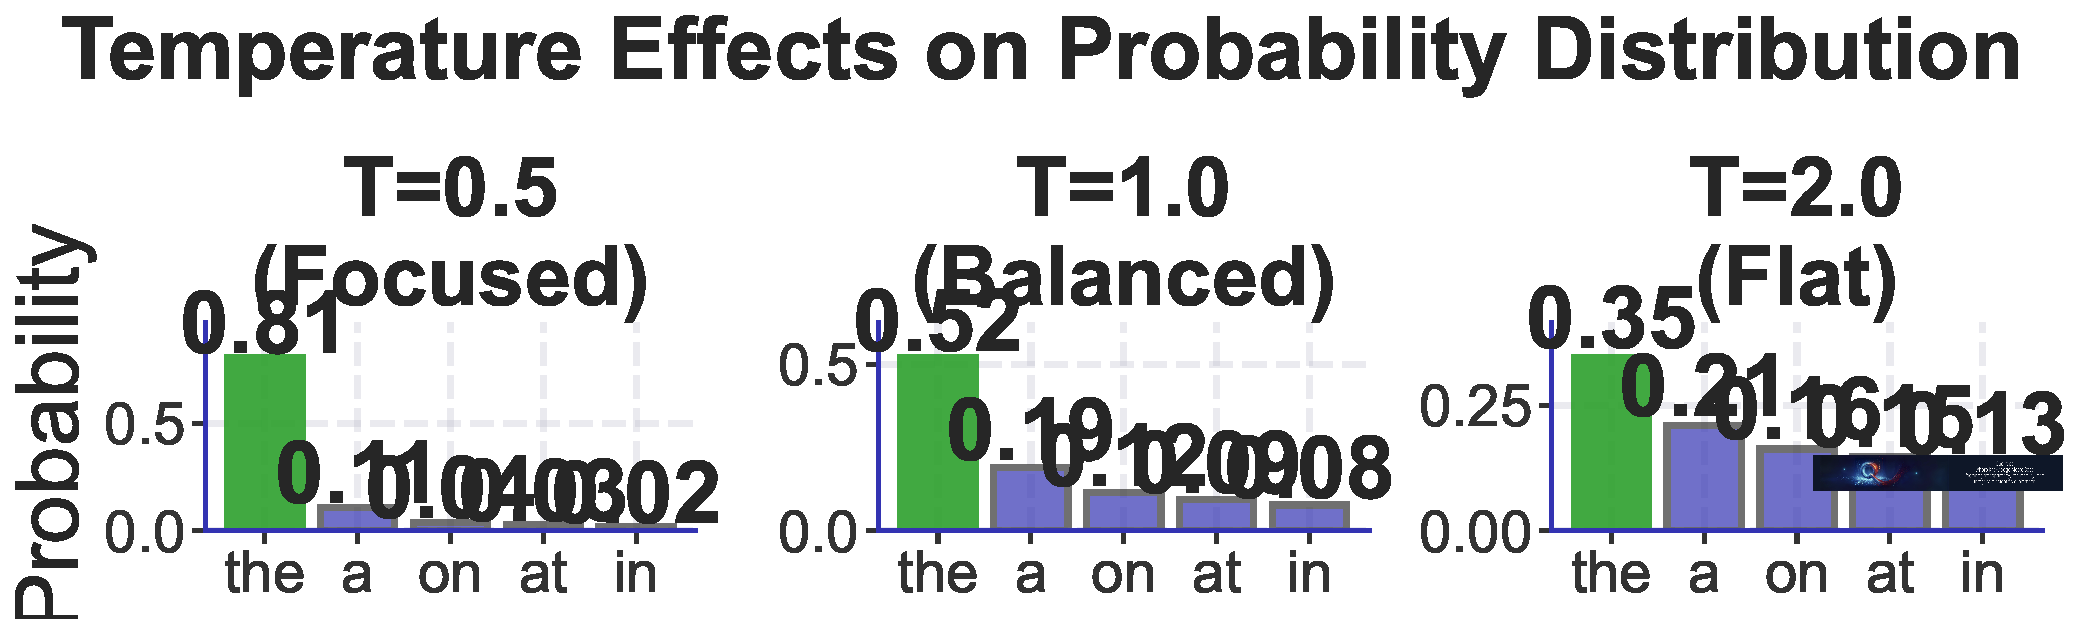
\includegraphics[width=0.85\textwidth]{../../figures/temperature_effects.pdf}
    
    \vspace{0.3em}
    \begin{columns}[T]
        \begin{column}{0.32\textwidth}
            \textbf{\textcolor{accent1}{Greedy}}
            \small
            \begin{itemize}
                \item Fastest
                \item Deterministic
                \item Can be repetitive
            \end{itemize}
        \end{column}
        \begin{column}{0.32\textwidth}
            \textbf{\textcolor{accent2}{Beam Search}}
            \small
            \begin{itemize}
                \item Better quality
                \item Multiple hypotheses
                \item More compute
            \end{itemize}
        \end{column}
        \begin{column}{0.32\textwidth}
            \textbf{\textcolor{accent3}{Sampling}}
            \small
            \begin{itemize}
                \item Creative
                \item Diverse outputs
                \item Temperature control
            \end{itemize}
        \end{column}
    \end{columns}
\end{frame}

\begin{frame}[t]{Week 9: Applications}
    \centering
    \includegraphics[width=0.85\textwidth]{../../figures/decoding_quality_metrics.pdf}
    
    \vspace{0.3em}
    \begin{columns}[T]
        \begin{column}{0.48\textwidth}
            \textbf{\textcolor{accent1}{Task Matching:}}
            \small
            \begin{itemize}
                \item Translation: Beam search
                \item Dialogue: Nucleus sampling
                \item Summarization: Greedy
                \item Creative: High temperature
            \end{itemize}
        \end{column}
        \begin{column}{0.48\textwidth}
            \textbf{\textcolor{accent2}{Parameters:}}
            \small
            \begin{itemize}
                \item Beam size: 4-10
                \item Temperature: 0.7-1.0
                \item Top-p: 0.9-0.95
                \item Length penalty
            \end{itemize}
        \end{column}
    \end{columns}
\end{frame}

%============================================================================
% WEEK 10: FINE-TUNING (3 slides)
%============================================================================

\section{Week 10: Fine-tuning}

\begin{frame}[t]{Week 10: Adaptation Techniques}
    \centering
    \includegraphics[width=0.85\textwidth]{../../figures/adaptation_decision_tree.pdf}
    
    \vspace{0.3em}
    \begin{columns}[T]
        \begin{column}{0.48\textwidth}
            \textbf{\textcolor{accent1}{What We'll Learn:}}
            \small
            \begin{itemize}
                \item Full fine-tuning
                \item LoRA/QLoRA
                \item Prompt engineering
                \item Prefix tuning
                \item Instruction tuning
            \end{itemize}
        \end{column}
        \begin{column}{0.48\textwidth}
            \textbf{\textcolor{accent2}{Challenges:}}
            \small
            \begin{itemize}
                \item Catastrophic forgetting
                \item Compute requirements
                \item Data efficiency
                \item Hyperparameter tuning
            \end{itemize}
        \end{column}
    \end{columns}
\end{frame}

\begin{frame}[t]{Week 10: Efficient Fine-tuning}
    \centering
    \includegraphics[width=0.85\textwidth]{../../figures/lora_explanation.pdf}
    
    \vspace{0.3em}
    \begin{columns}[T]
        \begin{column}{0.32\textwidth}
            \textbf{\textcolor{accent1}{LoRA}}
            \small
            \begin{itemize}
                \item Low-rank adapters
                \item 0.1\% parameters
                \item No inference cost
            \end{itemize}
        \end{column}
        \begin{column}{0.32\textwidth}
            \textbf{\textcolor{accent2}{Prompt}}
            \small
            \begin{itemize}
                \item Zero gradient
                \item Task instructions
                \item Few-shot examples
            \end{itemize}
        \end{column}
        \begin{column}{0.32\textwidth}
            \textbf{\textcolor{accent3}{Prefix}}
            \small
            \begin{itemize}
                \item Learnable prompts
                \item Task-specific
                \item Memory efficient
            \end{itemize}
        \end{column}
    \end{columns}
\end{frame}

\begin{frame}[t]{Week 10: Applications}
    \centering
    \includegraphics[width=0.85\textwidth]{../../figures/finetuning_vs_prompting.pdf}
    
    \vspace{0.3em}
    \begin{columns}[T]
        \begin{column}{0.48\textwidth}
            \textbf{\textcolor{accent1}{Domains:}}
            \small
            \begin{itemize}
                \item Medical NLP
                \item Legal documents
                \item Scientific papers
                \item Customer service
            \end{itemize}
        \end{column}
        \begin{column}{0.48\textwidth}
            \textbf{\textcolor{accent2}{Best Practices:}}
            \small
            \begin{itemize}
                \item Start with prompts
                \item Use LoRA for efficiency
                \item Validate thoroughly
                \item Monitor drift
            \end{itemize}
        \end{column}
    \end{columns}
\end{frame}

%============================================================================
% WEEK 11: EFFICIENCY (3 slides)
%============================================================================

\section{Week 11: Efficiency}

\begin{frame}[t]{Week 11: Model Optimization}
    \centering
    \includegraphics[width=0.85\textwidth]{../../figures/model_compression_landscape.pdf}
    
    \vspace{0.3em}
    \begin{columns}[T]
        \begin{column}{0.48\textwidth}
            \textbf{\textcolor{accent1}{What We'll Learn:}}
            \small
            \begin{itemize}
                \item Quantization (INT8/INT4)
                \item Knowledge distillation
                \item Pruning strategies
                \item Flash attention
                \item Model compression
            \end{itemize}
        \end{column}
        \begin{column}{0.48\textwidth}
            \textbf{\textcolor{accent2}{Goals:}}
            \small
            \begin{itemize}
                \item Reduce memory footprint
                \item Increase inference speed
                \item Lower latency
                \item Edge deployment
                \item Cost reduction
            \end{itemize}
        \end{column}
    \end{columns}
\end{frame}

\begin{frame}[t]{Week 11: Optimization Techniques}
    \centering
    \includegraphics[width=0.85\textwidth]{../../figures/quantization_levels.pdf}
    
    \vspace{0.3em}
    \begin{columns}[T]
        \begin{column}{0.32\textwidth}
            \textbf{\textcolor{accent1}{Quantization}}
            \small
            \begin{itemize}
                \item 4x memory reduction
                \item 2-3x speedup
                \item Less than 1\% accuracy loss
            \end{itemize}
        \end{column}
        \begin{column}{0.32\textwidth}
            \textbf{\textcolor{accent2}{Distillation}}
            \small
            \begin{itemize}
                \item 10x smaller
                \item Student-teacher
                \item Task-specific
            \end{itemize}
        \end{column}
        \begin{column}{0.32\textwidth}
            \textbf{\textcolor{accent3}{Pruning}}
            \small
            \begin{itemize}
                \item Remove weights
                \item Structured/unstructured
                \item 50-90\% sparsity
            \end{itemize}
        \end{column}
    \end{columns}
\end{frame}

\begin{frame}[t]{Week 11: Deployment}
    \centering
    \includegraphics[width=0.85\textwidth]{../../figures/deployment_pipeline.pdf}
    
    \vspace{0.3em}
    \begin{columns}[T]
        \begin{column}{0.48\textwidth}
            \textbf{\textcolor{accent1}{Platforms:}}
            \small
            \begin{itemize}
                \item ONNX Runtime
                \item TensorRT
                \item Mobile (Core ML)
                \item Edge devices
            \end{itemize}
        \end{column}
        \begin{column}{0.48\textwidth}
            \textbf{\textcolor{accent2}{Metrics:}}
            \small
            \begin{itemize}
                \item Throughput (QPS)
                \item Latency (p50/p99)
                \item Memory usage
                \item Power consumption
            \end{itemize}
        \end{column}
    \end{columns}
\end{frame}

%============================================================================
% WEEK 12: ETHICS (3 slides)
%============================================================================

\section{Week 12: Ethics \& Fairness}

\begin{frame}[t]{Week 12: Responsible AI}
    \centering
    \includegraphics[width=0.85\textwidth]{../../figures/ai_ethics_landscape.pdf}
    
    \vspace{0.3em}
    \begin{columns}[T]
        \begin{column}{0.48\textwidth}
            \textbf{\textcolor{accent1}{What We'll Learn:}}
            \small
            \begin{itemize}
                \item Bias detection
                \item Fairness metrics
                \item Privacy preservation
                \item Interpretability
                \item Robustness testing
            \end{itemize}
        \end{column}
        \begin{column}{0.48\textwidth}
            \textbf{\textcolor{accent2}{Key Issues:}}
            \small
            \begin{itemize}
                \item Dataset bias
                \item Demographic parity
                \item Harmful outputs
                \item Misinformation
                \item Environmental impact
            \end{itemize}
        \end{column}
    \end{columns}
\end{frame}

\begin{frame}[t]{Week 12: Bias and Fairness}
    \centering
    \includegraphics[width=0.85\textwidth]{../../figures/bias_sources.pdf}
    
    \vspace{0.3em}
    \begin{columns}[T]
        \begin{column}{0.32\textwidth}
            \textbf{\textcolor{accent1}{Sources}}
            \small
            \begin{itemize}
                \item Training data
                \item Annotation bias
                \item Model architecture
            \end{itemize}
        \end{column}
        \begin{column}{0.32\textwidth}
            \textbf{\textcolor{accent2}{Detection}}
            \small
            \begin{itemize}
                \item Demographic analysis
                \item Counterfactuals
                \item Probing tasks
            \end{itemize}
        \end{column}
        \begin{column}{0.32\textwidth}
            \textbf{\textcolor{accent3}{Mitigation}}
            \small
            \begin{itemize}
                \item Data augmentation
                \item Debiasing methods
                \item Fair objectives
            \end{itemize}
        \end{column}
    \end{columns}
\end{frame}

\begin{frame}[t]{Week 12: Future Directions}
    \centering
    \includegraphics[width=0.85\textwidth]{../../figures/fairness_techniques.pdf}
    
    \vspace{0.3em}
    \begin{columns}[T]
        \begin{column}{0.48\textwidth}
            \textbf{\textcolor{accent1}{Technical:}}
            \small
            \begin{itemize}
                \item Constitutional AI
                \item Alignment research
                \item Interpretable models
                \item Robust evaluation
            \end{itemize}
        \end{column}
        \begin{column}{0.48\textwidth}
            \textbf{\textcolor{accent2}{Societal:}}
            \small
            \begin{itemize}
                \item Regulatory frameworks
                \item Inclusive development
                \item Transparency standards
                \item Global cooperation
            \end{itemize}
        \end{column}
    \end{columns}
    
    \vspace{0.5em}
    \begin{tcolorbox}[colback=accent4!10,colframe=accent4,boxrule=0.5pt]
        \centering
        \small \textbf{Course Complete:} You're now ready to build responsible, state-of-the-art NLP systems!
    \end{tcolorbox}
\end{frame}

\end{document}